\section{Evaluation}

This section presents results and interpretations of four experiments designed to evaluate the performance and behavior of IFTD.  The questions explored by these experiments include:
\begin{enumerate}
\item How well can IFTD tolerate protocol errors in the active receiver scenario when the best protocol is unknown?
\item How much overhead does a lone receiver IFTD introduce into data transfers relative to other similar multiprotocol data transfer software?
\item How well can a lone receiver IFTD, using DCPs, maximize effective bandwidth relative to other, similar multiprotocol data transfer software?
\item If given time to learn, does the naive Bayes classifier in a lone receiver IFTD correctly identify the best data transfer protocol for prior labeled data feature vectors?
\end{enumerate}

These experiments were run on two single-processor machines on a gigabit copper switched LAN with no other network traffic present.  Each machine had an Intel\textsuperscript{\textregistered} Pentium\textsuperscript{\textregistered} 4 CPU clocked at 2.4 GHz with 2 GB of RAM, of which 1.25 GB was allocated to a RAM disk.  Each machine had an Intel(R) 82540EM gigabit Ethernet controller.  On each machine the files to transfer and the IFTD chunk directory were stored on the RAM disk so that the time-dependent experiments would not be affected by disk I/O operations.

\subsection{Protocol Fault Tolerance}

\begin{figure}[h!]
    \centering
    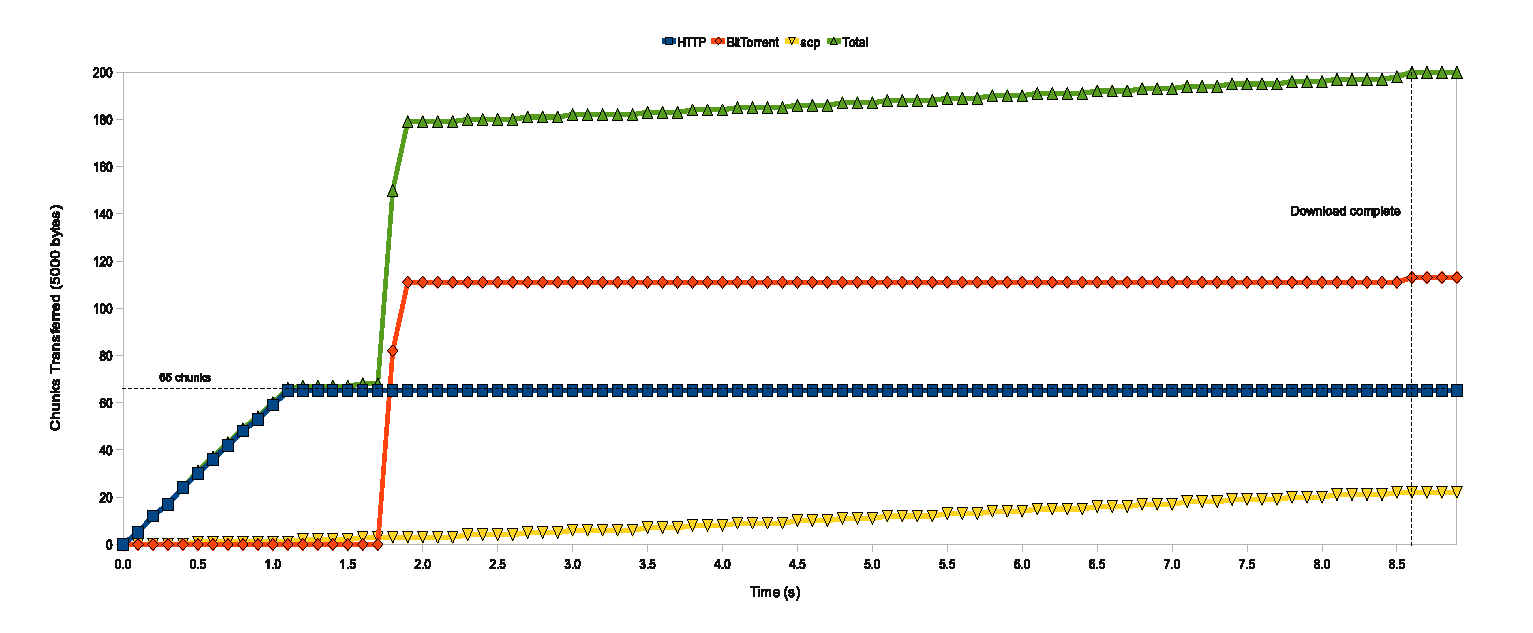
\includegraphics[width=1.0\textwidth]{diagrams/protocol-fault-toleration}
    \caption{Number of chunks transferred by each protocol as a function of time.  The HTTP protocol is programmed to transfer 65 chunks and fail, while the BitTorrent and scp protocols continue to receive the remaining 135 chunks.}
    \label{protocol-fault-toleration}
\end{figure}

An important aspect of a multiprotocol data transfer service is how well it can tolerate errors in single protocols.  The purpose of this experiment is to demonstrate how well IFTD can tolerate protocol failures by measuring how many chunks each available protocol transfers at different times during a transfer.  For this experiment the local IFTD is configured to use three protocols to receive a million-byte file that has been broken into 200 evenly-sized chunks by a remote IFTD.  The first protocol uses the \texttt{scp} binary to retrieve chunks from the remote host.  The second protocol uses the Rasterbar libtorrent library~\cite{libtorrent} to retrieve pieces of the file from a BitTorrent swarm, where the remote IFTD is a seed for the file.  The third protocol uses \texttt{http} to retrieve chunks from the remote host, but is programmed to arbitrarily fail after receiving 65 chunks.

The protocol usages are summarized in Figure~\ref{protocol-fault-toleration}.  Upon execution, the HTTP protocol will reserve a chunk, retrieve it, write it, and repeat the process 65 times before failing.  The \texttt{scp} protocol runs concurrently with the HTTP and BitTorrent protocols, but since it must perform public/private key encryption to begin receiving each chunk, it receives data at a much slower rate than the other two.  The BitTorrent protocol takes longer to start receiving--longer than it takes the HTTP protocol to receive all of its pre-programmed chunks--but once it learns the IP address of the remote host from the BitTorrent tracker, it quickly receives most of the data and concurrently stores them alongside the \texttt{scp} protocol.  It contacts the remote IFTD periodically for more chunks and receives a few more at nearly 8.4 seconds into the transmission.

The local IFTD does not have any prior information with which to train its classifier, so it receives data using all three protocols concurrently.  Consequently, the behavior demonstrated here is typical only when IFTD has not performed enough transfers to initialize its classifier.

Since the BitTorrent receiver implementation is an NCP and does not know in advance which chunks will be sent to it, it receives many duplicate chunks relative to the HTTP and \texttt{scp} receivers.  In fact, it received two chunks that the \texttt{scp} protocol, a DCP, had reserved and was in the process of downloading.  The duplicated effort resulting from using BitTorrent alongside HTTP and \texttt{scp} is summarized in the following table.


\begin{table}[ht!]
\centering
\begin{tabular}{ | l | l | l | l | }
\hline
 & HTTP & BitTorrent & \texttt{scp} \\
\hline
Chunks Saved & 65 & 113 & 22 \\
Chunks Re-downloaded & 0 & 86 & 2 \\
\hline
\end{tabular}
\caption{How many chunks were written versus how many chunks were rejected by the chunk reservation system using the protocols in Figure~\ref{protocol-fault-toleration}.}
\label{protocol-effective-bandwidth}
\end{table}

Duplication notwithstanding, this experiment demonstrates that IFTD can tolerate a complete protocol failure and continue to receive data.  The application for which IFTD performs a transfer does not need to implement any logic for handling such errors.

\subsection{Transfer Overhead}

\begin{figure}[h!]
    \centering
    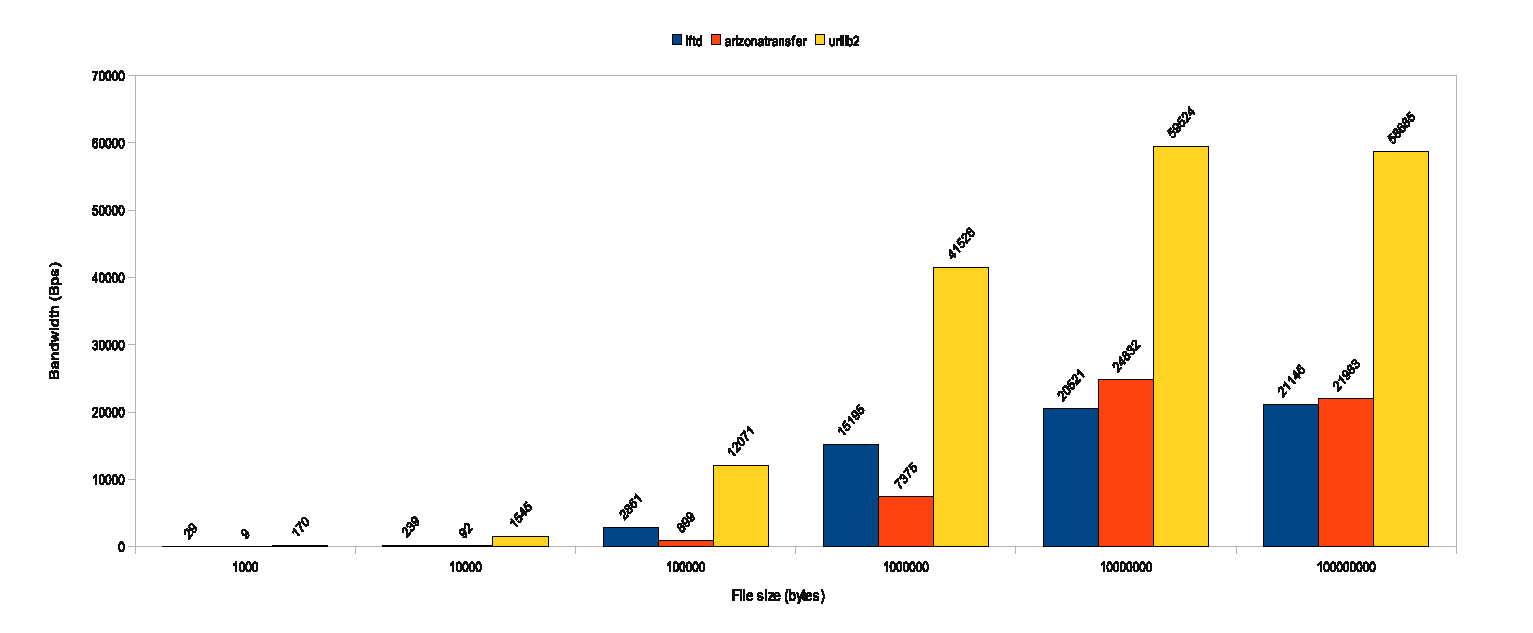
\includegraphics[width=1.0\textwidth]{diagrams/transfer-overhead}
    \caption{Bandwidth as a function of file size.  Because all three pieces of software transfer data across a gigabit LAN, the affect of transfer overhead on each piece of software's bandwidth is noticeable for files less than 10MB in size.}
    \label{transfer-overhead}
\end{figure}

One consideration in choosing a multiprotocol data transfer service is the measure of how much overhead each service adds to an application's transfer processing.  This experiment demonstrates how fast IFTD retrieves a file from a remote host relative to arizonatransfer and \texttt{urllib2}.  All three pieces of transfer software retrieved files from a CherryPy 3.1.2 HTTP server~\cite{cherrypy}, and were given the file's size in advance.  IFTD used only its HTTP protocol, received only from CherryPy, and retrieved each file as a single chunk\footnote[4]{In implementation, this allowed IFTD's HTTP protocol to avoid performing byte-range GETs, making it comparable to arizonatransfer and \texttt{urllib2}.}.

The data in Figure~\ref{transfer-overhead} represent the average of 10 consecutive transfers for each piece of transfer software for a range of file sizes.  The bandwidth was calculated as the file size divided by the amount of time spent setting up, receiving data from, and shutting down a connection to the remote host.  In IFTD, the amount of time measured is the round-trip time for an XMLRPC call to IFTD's \texttt{begin\_ift()} method.  In arizonatransfer, the amount of time measured is the time taken for the call to the \texttt{getfiles1()} method to complete.  In \texttt{urllib2}, the amount of time measured is the time taken for opening a new file, calling the \texttt{urlopen()} method to contact the remote host, calling the \texttt{read()} method on the \texttt{Response} object returned by \texttt{urlopen()} to receive all the data, writing the data to the file, and closing the file.  In the first two cases, file integrity checking is disabled.

Predictably, \texttt{urllib2} retrieved all files faster than arizonatransfer and IFTD.  This is because the method used to receive data in a \texttt{urllib2} \texttt{Response} object is mapped directly to the Python socket package's \texttt{recv()} method~\cite{urllib2_code}, which in turn calls the POSIX \texttt{recv()} function with the actual socket descriptor in Linux to receive data from the remote host.  Also, unlike arizonatransfer and IFTD, an application that uses \texttt{urllib2} supplies the protocol and URL that identify the way in which to receive data, thus freeing \texttt{urllib2} from the responsibility of determining which protocol to use.  Consequentially, there is much less overhead in transferring data using \texttt{urllib2} than with arizonatransfer and IFTD, because the latter two must identify which protocol(s) to use before they can begin transferring data.

For files less than 10MB in size, IFTD has a higher bandwidth than arizonatransfer.  This is partly because arizonatransfer loads and initializes its transfer protocol modules each time an application calls its \texttt{getfiles1()} method, and because it receives data to a temporary file which is then moved to the application's requested destination path using the Python \texttt{shutil} package.  IFTD does neither of these; instead, it loads and initializes its protocols only once when it starts up and writes data chunks directly to the destination path.  Consequently it has better performance for smaller files, even though using it incurs the cost of an XMLRPC round-trip.

When processing files on the order of 10MB, IFTD is noticeably slower than arizonatransfer.  Although the data show that IFTD is still slower than arizonatransfer at transferring files on the order of 100MB, the difference in bandwidth for 100MB files is significantly less than it is for 10MB files.  The reasons for this are unclear.

Even though \texttt{urllib2} had the highest bandwidth in all cases, the data show that IFTD was able to maintain bandwidths comparable to arizonatransfer.  This suggests that IFTD may be a suitable replacement for arizonatransfer in the Stork package manager.


\subsection{Recoverability Performance}

\begin{figure}[h!]
    \centering
    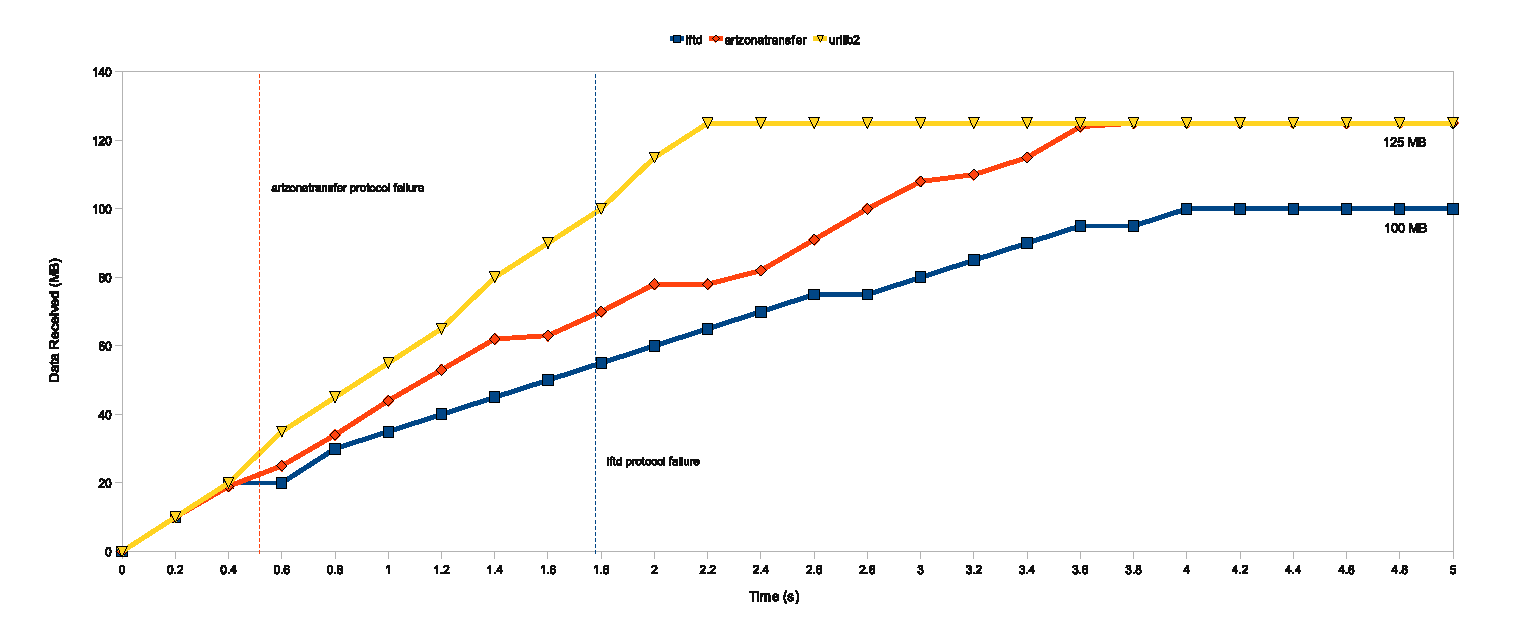
\includegraphics[width=1.0\textwidth]{diagrams/recoverability-performance}
    \caption{Number of bytes received by each data transfer software as a function of time when a 100 MB file is re-requested after one fourth of it downloads.  Although \texttt{urllib2} and arizonatransfer have higher bandwidths than IFTD, they transfer more data than IFTD since they are not resumable.}
    \label{recoverability-performance}
\end{figure}

When the unit cost of moving data across a network is nontrivial, data transfer resumability and recoverability become desirable features in a transfer service.  The purpose of this experiment is to measure how much data is transferred over time when both arizonatransfer and IFTD use two different HTTP protocol implementations, one of which is programmed to fail after transferring one fourth of the requested data.  Both arizonatransfer and IFTD are expected to tolerate this protocol error and continue to receive data.  Arizonatransfer is expected to fail over to its next available protocol and in doing so re-transfer the first fourth of the data, whereas IFTD is expected to use its still-operational protocol to receive only the remaining three-fourths of the data.  At each 0.2 second interval, the experiment measures how much data arizonatransfer and IFTD were able to download with one faulty HTTP protocol implementation.  The total amount of data to transfer is 100 million bytes.  IFTD's chunk size was 5 million bytes.  The remote host used CherryPy 3.1.2 to serve data via HTTP on two different ports.

For comparison, the experiment calculated the amount of data transferred by \texttt{urllib2} when using \texttt{urllib2} to set up a connection to the remote host, transfer 25 million bytes, close the connection, re-open the connection, transfer all 100 million bytes, write the data to disk, and close the connection again.  The reason for this particular behavior is to emulate the behavior of a hypothetical application that repeatedly attempts to receive data with \texttt{urllib2} by re-requesting the data if the previous transfer request fails.  In this scenario, the first transfer request fails after receiving 25 million bytes, and the second request succeeds in receiving all 100 million bytes (meaning that the application transfer 125 million bytes before successfully receiving the data).

The times of arizonatransfer's and IFTD's protocol failures are indicated in Figure~\ref{recoverability-performance} with vertical bars.  IFTD receives 100 million bytes, whereas both \texttt{urllib2} and arizonatransfer receive 125 million as expected.

IFTD only receives 100 million bytes and encounters the error after receiving 50 million bytes because it concurrently uses both its faulty and operational HTTP protocol implementations to receive data in 5 million byte chunks.  By the time its faulty HTTP implementation fails, both it and the operational HTTP implementation will have received 25 million bytes each.  IFTD uses the operational HTTP implementation to receive the remaining 50 million bytes of the file, despite the failure of the faulty HTTP implementation.

In this experiment, the data show that IFTD's protocol architecture and fault tolerance give it the ability to use DCPs like HTTP to avoid re-transferring data that has already been received from a remote host without IFTD.  This resumability allows an application to receive less data than it would have with arizonatransfer or this particular usage of \texttt{urllib2} in the event of one or more protocol errors.

\subsection{Protocol Classification}

\begin{figure}[h!]
    \centering
    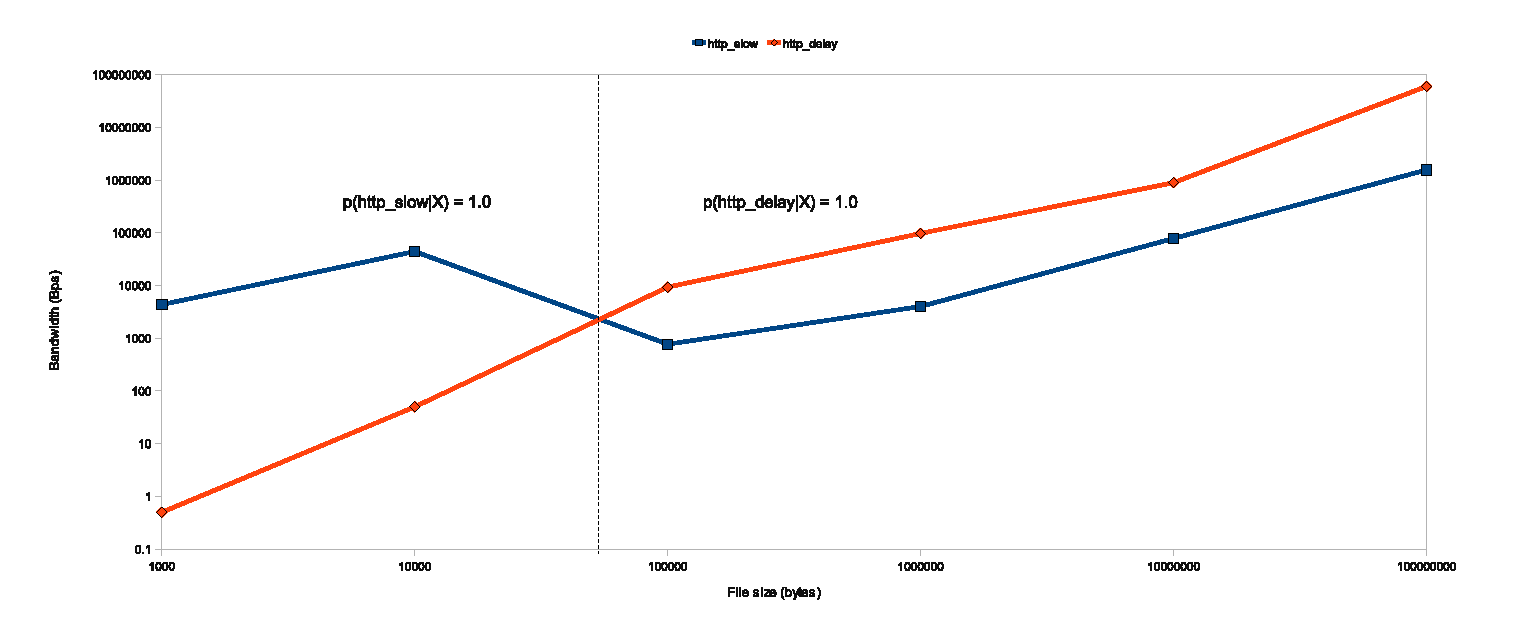
\includegraphics[width=1.0\textwidth]{diagrams/protocol-classification}
    \caption{The IFTD-measured bandwidths of two different HTTP implementations for different file sizes.  IFTD chooses \texttt{http\_slow} for smaller files since it has a higher average bandwidth than \texttt{http\_delay} for small amounts of data.  IFTD chooses \texttt{http\_delay} over \texttt{http\_slow} once the files become big enough that transferring it with \texttt{http\_delay} is faster.}
    \label{protocol-classification}
\end{figure}

One benefit of using a classifier to select the best protocol for a data transfer is that it allows IFTD to choose low-latency but low-bandwidth protocols to transfer small amounts of data, and high-latency but high-bandwidth protocols to transfer large amounts of data.  In this experiment, IFTD uses two different HTTP implementations to transfer data of various sizes from a remote HTTP server.  The first HTTP implementation, \texttt{http\_slow}, is programmed to receive data as fast as possible for small files, but to introduce a sharp, artificial delay for each chunk proportional to the inverse of the file size when transferring large files.  The second HTTP implementation, \texttt{http\_delay}, is programmed to wait 10 seconds before receiving data and then to receive data as fast as possible.  Their bandwidths, calculated as an average of 10 consecutive transfers for each given file, are plotted in Figure~\ref{protocol-classification} on a logarithmic bandwidth scale to emphasize the point where \texttt{http\_delay}'s bandwidth exceeds \texttt{http\_slow}'s bandwidth.  For the purpose of this experiment, IFTD is configured to refine its classifier after every 10 transfers.

After the experiment transfers each file 10 times from the remote host, it checks the probabilities of each protocol given the data feature vector.  The experiment always chooses a chunk size for IFTD to guarantee that there will be 20 evenly-sized chunks to transfer.  The probabilities of each protocol given the data features correlate strongly with the protocol with the highest average bandwidth for that data--in this case, the probability of either protocol given the data feature vector is either 0.0 or 1.0, depending on which received the most data for each set of transfers.

To summarize, in this experiment the data show that IFTD can detect and correctly associate small data transfers with a low-latency, low-bandwidth protocol and large data transfers with a high-latency, high-bandwidth protocol.  The probabilities of both protocols being the best for the transfer given the data correlate with the prior bandwidths IFTD had measured while using them.

